\chapter{Background}\label{s:background}
%\todo{This section provides the necessary context to help the reader understand the remainder of the thesis.}
\section{Problem definition}
One of the main objectives of the Digitale Overheid (Digital Government) is to 'Protect fundamental rights and public values' \cite{DO_agenda}. One could argue protecting the identity and privacy of citizens is part of this objective. The objective of this research is to mitigate the opportunity of identity theft and simultaneously improve citizens’ privacy by making use of appropriate information systems.

\subsection{Grounds for this research}
The Unique Identity Number (UIN) of the Dutch citizen is the ‘Burger Service Nummer’, abbreviated by BSN. In English this means ‘Citizen Service Number’. It’s comparable with the Social Security Number in the USA and it is also being applied to identify a person within Dutch governmental organizations and other parties who are legally permitted to use the BSN. \par
The World Bank \cite{WorldBank_UIN} positions UINs or equivalent ID numbers in the context of "foundational systems". ID numbers are considered to be unique when: firstly, the number-generating process ensures that no two people within the system share the same number and secondly, a deduplication process ensures that the same person does not have multiple identity records or numbers (i.e., that they are unique in the database)." The World Bank identifies two derived strengths, namely ‘Uniqueness and deduplication’ and ‘Data matching and interoperability’. This means each person can be identified uniquely, allowing for a fast and easy exchange of identity related information between different organizations.\par 
However, the benefit of fast and easy exchange of identity related information, is also highly susceptible to misuse. Identity Fraud and Theft leans heavily on the benefit of ‘Data matching and interoperability’ of the UIN. A second form of misuse that leans on this benefit is Unauthorized Data Correlation. \par
The Dutch governmental audit service, Auditdienst Rijk (ADR) defined gaps and possible improvements in usage of this number\cite{ADR}. This report discusses one of the advantages of BSN being a unique identifier for many different government and non-government organizations. Carrying out their administration more efficiently. Another obtained objective with the introducing of BSN was to prevent identity fraud. Facts and figures in the report of ADR are showing Identity Fraud is a growing issue over the last years. An illegally obtained BSN can be misused to impact the privacy of citizens negatively, while on the other hand the BSN has advantages within the Dutch government. The same BSN is re-used for different purposes. For example, a bank uses the same BSN of a citizen as does a hospital. If the hospital would have a data breach, this BSN could be re-used when committing identity fraud, for example at a bank. However, solely having the BSN without other personal information is not enough to commit identity fraud . During the design-phase of this research it was the assumed that identity theft has a creal definition and the BSN is merely an attribute of personal information to focus on. However, after initiating this research it has become clear that the BSN is only a part of the problem, and that a clear definition of identity theft is required in order to prevent different viewpoints of the researched problem, when discussing possible solutions. Quantifying and scoping this broad problem into an operational problem, will facilitate the discussion on possible and appropriate solutions in information systems. \par

\section{Scope} \label{scope}
To correctly frame the problem and possible solutions it is needed to have clear definitions and a clear scope of the problem. Besides a UIN, there are more attributes of personal identity that are linked to an individual person. The 'UK national fraud and cybercrime reporting centre' states that only a name, date of birth and current or previous addresses could already be used to commit identity fraud.\cite{Action_fraud}. One way to obtain this identity data is through data breaches, for example a breach via commercial parties or (semi-)government. Recent examples are Booking.com \cite{Booking_databreach} or the Dutch GGD \cite{GGD_databreach}.

This section will describe how to frame the position of a UIN among other data within the domain of identity data.
De Vries \etal \cite{Vries2007IdentiteitsfraudeEA} split up identity fraud in two domains: 'Means of identification' (for example a passport or drivers licence) and 'Identity data'. Obviously identity fraud applies to both domains. However, because of restrictions in time and resources the scope of this research will only on the domain of 'Identity data'.
Figure \ref{fig:ID_domain} decomposes the domain of 'Identity data' described by De Vries \etal. This research will narrow its scope further to 'Formal functional identity data'. Formal functional identity data can be used in the part of 'Profile data' and therefore considered as an applications of 'Identity data' within this research.  A UIN as assigned identity data can be used in this profile by facilitating combination of data sets and possible unauthorized profiling. Definitions provided by De Vries \etal: 

    \begin{figure}
        \graphicspath{ {./images/} }
        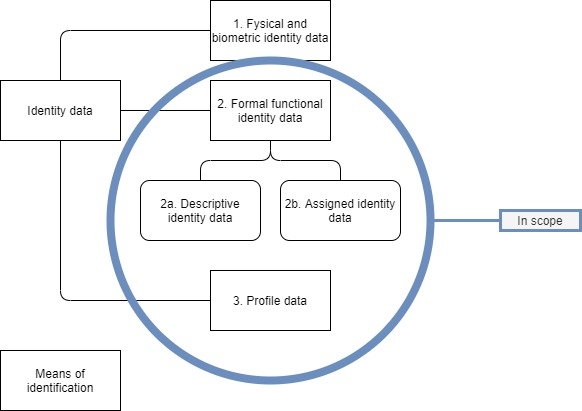
\includegraphics[width=10cm]{Identity data definitions and domain-Overview.jpg}\\
        \caption{Domain and scope of Identity Data - De Vries \etal \cite{Vries2007IdentiteitsfraudeEA}}
        \label{fig:ID_domain}
    \end{figure}

\begin{enumerate}
\item \textit{Physical and bio-metric identity data} - General physical identification data. For example sex, height, hair color, iris, DNA-profile or medical history
% Spelling komt niet overeen met plaatje. Zowel de F/PH als het streepje bij bio-metric
\item \textit{Formal functional identity data} - Data assigned or ascribed in a certain stage of phase of life of an individual person. To functionally distinguish individuals and assign rights and obligations to this individual.
\begin{enumerate}
\item \textit{Descriptive identity data} - Data that describes a person and the persons surroundings. Information that is close to the individual and is factual and mostly static. For example, family name, parents, place of birth, date and time of birth. 
\item \textit{Assigned identity data} - Data that is assigned and mostly describes a (contractual) relationship with organisations to provide products and services.
\end{enumerate}
\item \textit{Profile data} - Based on a certain set of factual data, an algorithm defines profiles that categorize a person. 
\end{enumerate}

\subsection{Definition of Identity Fraud}\label{Def_ID_Fraud}
After commencing this research it became clear Identity Fraud is a catch-all term and a clear definition supports a clear scope. De Vries \etal \cite{97408536fd1c4f4e9d1615b7a4a4473e} have analysed 30 international definitions and formulated the following general description "Identity Fraud is to obtain, to possess or to create intentionally, (and) (unlawfully or without consent) false means of identification in order to commit unlawful behaviour, or to have the intention to commit unlawful behaviour." In the footnote it states: "It must be noted that ‘false’ in the description refers to the idea that the means of identification do not identify the person who uses them truthfully." 
Figure \ref{fig:ID_fraud} shows the different types of mismatch between a person and identity data, defined by De Vries \etal \cite{Vries2007IdentiteitsfraudeEA}. The three items marked blue define the focus for this research, namely Identity Theft.

    \begin{figure}
        \graphicspath{ {./images/} }
        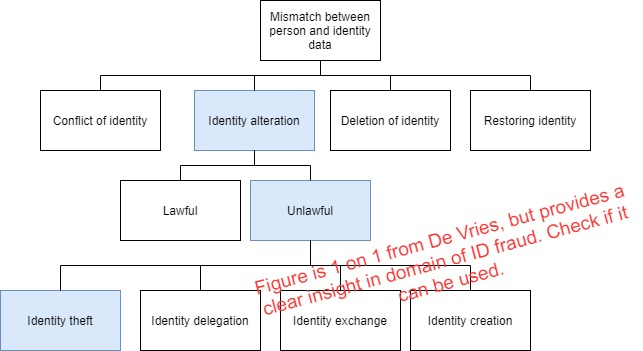
\includegraphics[width=10cm]{Domain of Identity fraud.jpg}\\
        \caption{Domain and scope of Identity Fraud - De Vries \etal \cite{Vries2007IdentiteitsfraudeEA}}
        \label{fig:ID_fraud}
    \end{figure}

\subsection{Quantitative impact of Identity Fraud}\label{QI}
De Vries \etal claim that it is difficult to quantify identity fraud because it is incorporated in other crimes\cite{Vries2007IdentiteitsfraudeEA}. Goudriaan \etal claim many crimes in Western countries are not even reported to the police \cite{Gourdriaan_etal}. This research bases quantification of the problem on statistical resources and reports. Quantification is relevant to define the impact of the problem and for purposes of raising awareness and having a generic view on the problem. To quantify the impact of the solutions it is required to define the methods and means of measuring the impact after implementation. Due to time and capacity restrictions, the quantification of the impact is out of scope. The impact of possible solutions will be based on logical reasoning and argumentation.

The Auditdienst Rijk (ADR)\cite{ADR} has generated a report taking into account facts of the 'Citizen service for Identity Fraud' at the 'National Office for Identity Data' (Rijksdienst voor Identiteitsgegevens). Somewhere around 4.000 citizens a year contact this service to report identity fraud. In some cases the impact is low and only a discomfort. In other cases the fraud results in identity theft that can lead to crimes committed by fraudsters in name of that person. Resulting in fines or debts wrongfully matched with the victim.\par 

Statistics Netherlands (CBS) quantified data of identity fraud based on statistical data \cite{CBS_DigitaleVeiligheid}. Purely looking at the data classified by Identity Fraud, CBS defines it: "Without permission, via internet, making use of someones personal data for financial gain, for example by withdrawing or transferring money, taking out a loan or requesting official documents." Roughly 0.5\% of Dutch citizens in 2019 became victim of identity fraud. 0.1\% repeatedly became victim. Based on a population of 17 million, this means roughly 86.000 people are confronted with Identity Fraud each year. 17.000 of them are repeated victims. Figure \ref{fig:CBS_Total_ID_fraud} and Figure \ref{fig:CBS_ID_fraud} show the numbers and how it's divided throughout The Netherlands.

    
    \begin{figure}
        \graphicspath{ {./images/} }
        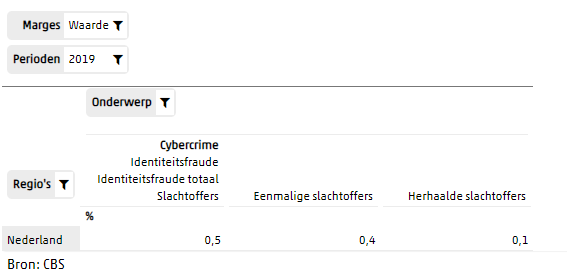
\includegraphics[width=7cm]{Cybercrime - identiteitsfraude Nederland totaal.png}\\
        \caption{Victims of Identity Fraud \cite{CBS_IDFraudTable} as a percentage of the total Dutch population in 2019 (17.282.163 \cite{CBS_totalpopulation2019}) - CBS}  
        \label{fig:CBS_Total_ID_fraud}
    \end{figure}

    
    \begin{figure}
        \graphicspath{ {./images/} }
        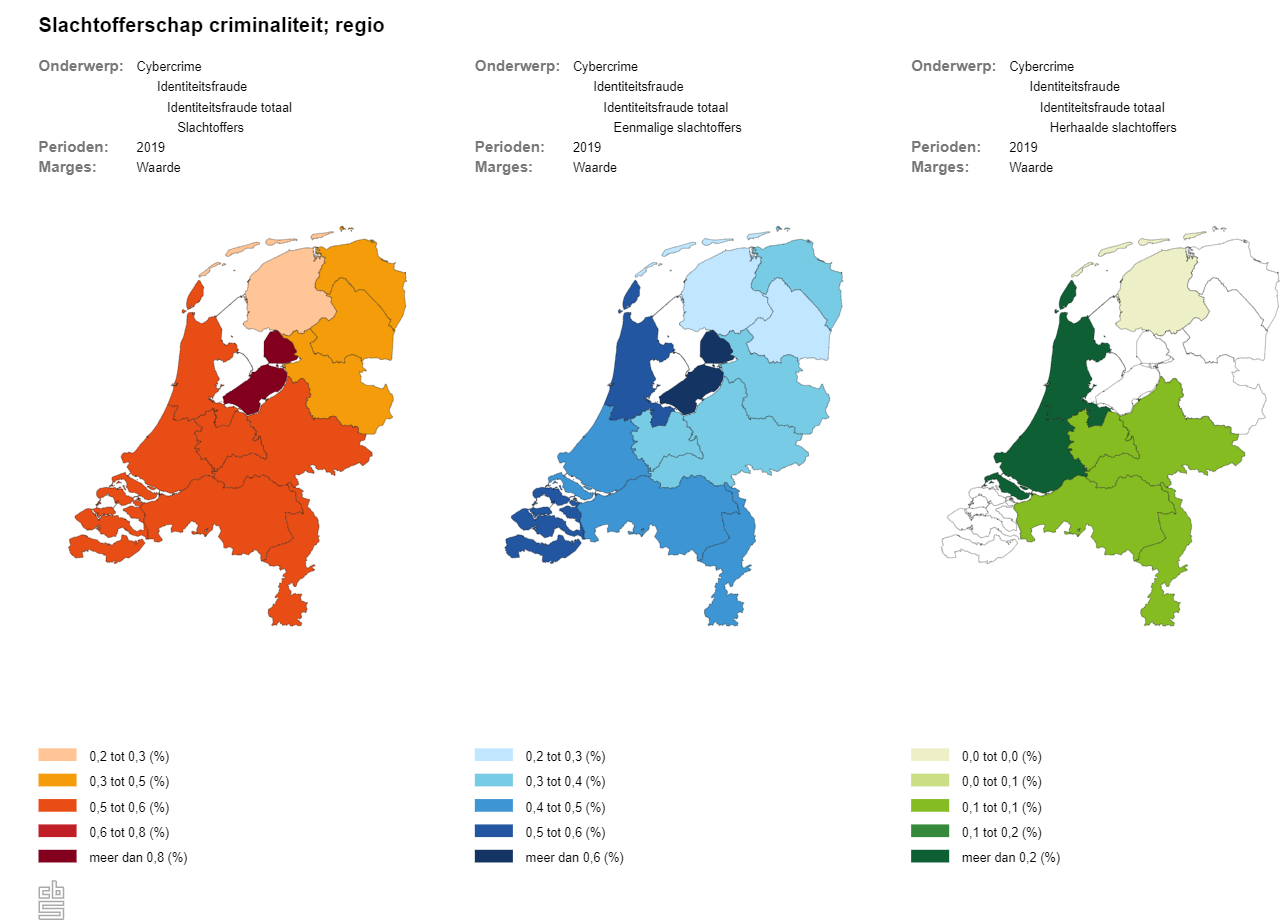
\includegraphics[width=12cm]{Slachtofferschap_delicten__regio__29012022_145152.png}\\
        \caption{Division per Province  \cite{CBS_IDFraudTable} - CBS}  
        \label{fig:CBS_ID_fraud}
    \end{figure}

Another research of the CBS focuses on the impact categorization of victims {\cite{CBS_casualtiesDigitalCrime}}. Concluding property crime as the most victimized crime. 

\subsection{Personal Records Database (BRP) and data provisioning}\label{BRP}
The Dutch Personal Records Database or Basisregistratie Personen (BRP) contains personal information (including BSN) and history of a person in a list of attributes. BRP contains attributes of Formal functional identity data of both residents and non-residents. Residents are citizens residing in a municipality for a consecutive period. Non-residents are citizens temporarily living or working within The Netherlands or citizens with Dutch nationality who live abroad. \cite{BRP} The BRP provides a selection of attributes or a complete list with attributes of identity data which an organizations is permitted to acquire by law. The provisioned data is then replicated to the database managed by that organization. From the perspective of data minimization, organizations will have to minimize the provided content for the purpose of use.  

\subsection{Operational problem}\label{OP}
The World Bank ID4ID defines vulnerabilities and risks when UINs are ubiquitously available \cite{WorldBank_protecting}. Identity fraud and unauthorized data correlation are two operational problems. This research will focus on possible practical solutions applied to the BRP with a focus  on 'Profile data' by using 'Formal functional identity data' as defined in section \ref{Def_ID_Fraud}. UIN and other attributes of a person can be defined as 'Assigned identity data'. Architectural patterns and tactics will be used to help mitigate the operational problems, taking relevant QA's and ASRs into account. Concretely, providing and replicating identity information could result in unforeseen misuse. Part of the possible solutions in Section \ref{s:Implementation} of this research is to minimize provided data. One of the additional practical problems could be lawfully mandated sharing of personal data sharing from the BRP. Having to take this in account when designing solutions.